\section{Diverse Failure Modes in Long Chain-of-Thought Reasoning} \label{sec: unreliable visual perception in long-chain reasoning}

\begin{figure}[t]
    \centering
    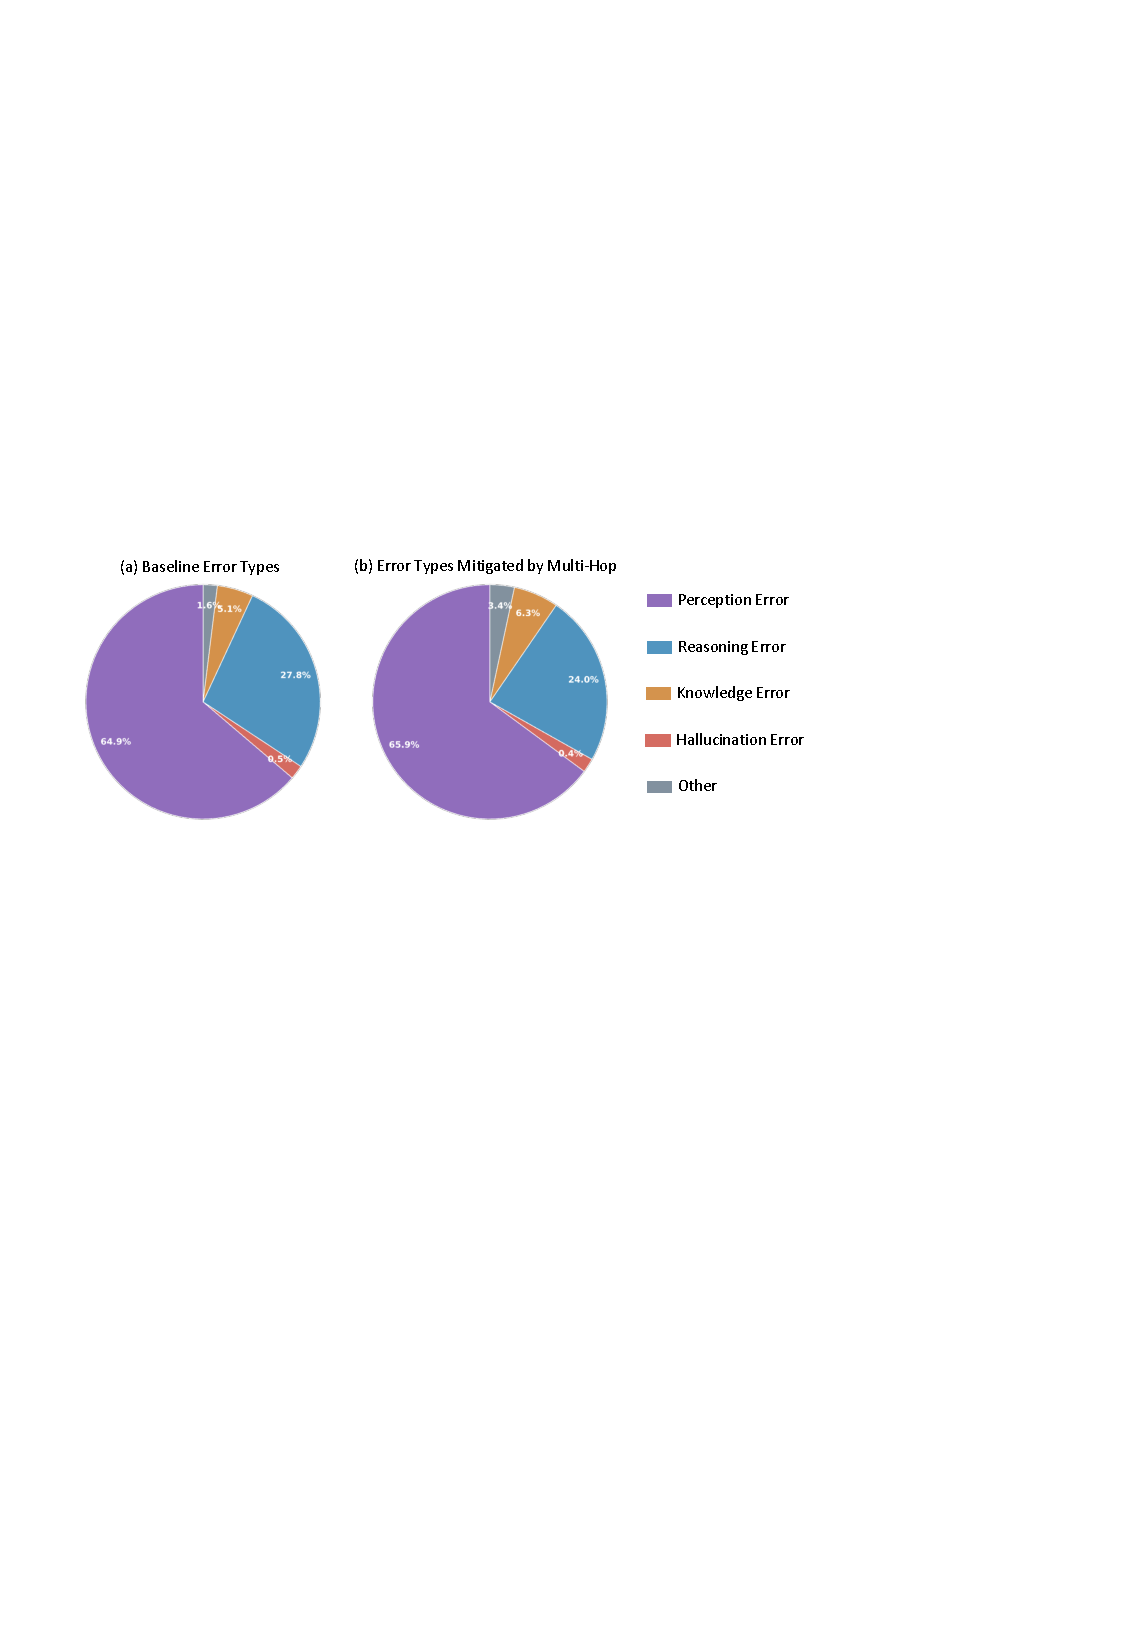
\includegraphics[pagebox=cropbox,width=0.8\textwidth]{imgs/error_distribution_new_2.pdf}
    \caption{Error-type distributions before and after adding multi-hop data in RLVR. Subfigure (a) shows the error-type distribution of \texttt{RLVR w/o Multi-Hop} on the benchmarks in Tables~\ref{tab:exp-35b} and~\ref{tab:exp-397b}. Subfigure (b) shows the distribution of baseline error types mitigated after adding multi-hop data (i.e., cases corrected by \texttt{RLVR w/ Multi-Hop}). In (a), errors are diverse, with perception and reasoning errors as the dominant categories. In (b), the distribution remains similar to (a), indicating that multi-hop data mitigates failures in a generalizable way rather than improving only a narrow error type. \Cref{fig:qualitative_examples} provides representative perception reasoning failures, together with responses corrected after adding multi-hop data.}
    \label{fig:error_distribution}
\end{figure}

Long CoT reasoning places a much higher demand on visual grounding than short, single-step QA.
To answer correctly, a VLM must repeatedly return to the image, recover the right object, attribute, relation, or numeric evidence at each step, and use that evidence to determine the next step of reasoning.
This makes long CoT reasoning inherently fragile: multiple error types can emerge along the chain, including perception, reasoning, knowledge, and hallucination errors, among others.
Once any such error appears at an intermediate step, the remaining reasoning can still look coherent while operating on flawed intermediate evidence, eventually producing an incorrect final answer.
Recent analyses in multimodal reasoning report similar patterns: longer reasoning traces can drift away from image-grounded evidence, reduce attention to visual inputs, and amplify hallucinated intermediate content~\CiteParen{liu2025morethinking,luo2025thinkingdrifts}.
More generally, diagnostic studies of VLMs have also documented persistent object hallucination and visual illusion under image-context reasoning~\CiteParen{rohrbach2018object,guan2024hallusionbench}.



\begin{figure}[!h]
    \centering
    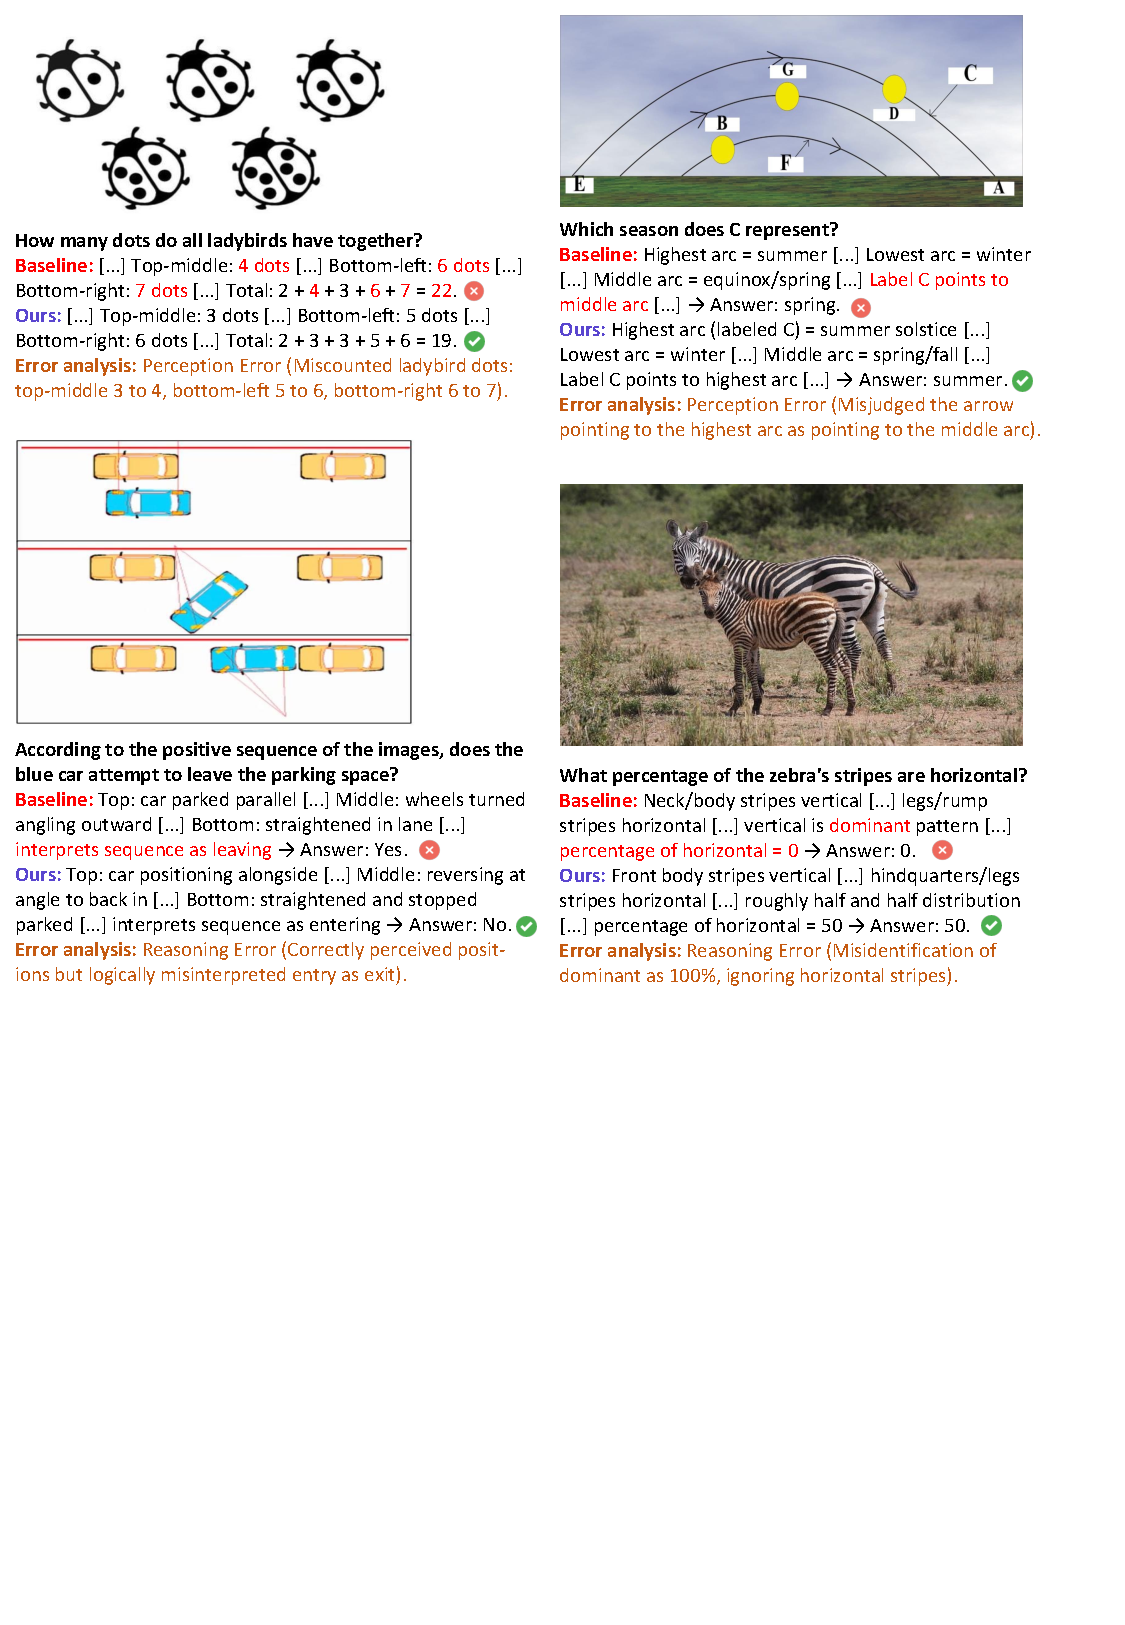
\includegraphics[width=1\textwidth]{imgs/qualitative_examples_new_5.pdf}
    \caption{Qualitative examples of unreliable visual perception in long CoT reasoning. We show failure cases from the benchmarks in \cref{tab:exp-35b,tab:exp-397b} using ``RVLR w/o Multi-Hop'' (baseline), alongside correct answers from ``RVLR w/ Multi-Hop'' (ours). For brevity, unimportant parts of the long CoT are omitted with $[\dots]$. The baseline error is highlighted in red, and the failure reason is given in the error analysis.}
    \label{fig:qualitative_examples}
    \vspace{-5pt}
\end{figure}


To obtain the error breakdown in \cref{fig:error_distribution}, we analyze responses produced on the benchmarks in \cref{tab:exp-397b} by Qwen3.5-397B-A17B under the \texttt{RLVR w/o Multi-Hop} setting. For each benchmark, we randomly sample 20 incorrect responses and ask annotators to identify the primary failure type by comparing the model output against the ground-truth answer.
The resulting breakdown shows that long-CoT failures are diverse rather than concentrated in a single category: perception errors are the largest group, while reasoning, knowledge, and hallucination errors are also present in the breakdown.
Qualitative examples in \cref{fig:qualitative_examples} further show that these failures are not limited to a narrow benchmark type.
The baseline model (\texttt{RLVR w/o Multi-Hop}) miscounts small local details in the ladybird example, misjudges the contact relation between the gripper and the dress strap, misreads the sign shape in the driving scene, reads chart values incorrectly, follows the wrong arc in the astronomy diagram, and selects the wrong body part in the fish illustration.
These examples cover natural images, charts, and scientific diagrams, but they share the same structure: one faulty intermediate step appears in the middle of a long reasoning chain, and the later reasoning steps inherit that mistake.
In this sense, long-CoT errors are often coupled rather than isolated: a mistaken visual judgment can trigger faulty reasoning, unsupported inference, or other downstream failures.
By contrast, \texttt{RLVR w/ Multi-Hop} is more likely to recover the correct visual evidence at each hop and therefore reaches the correct final prediction.

This analysis suggests that the central challenge is not merely producing a longer textual CoT, but maintaining reliable, step-wise reasoning over visual evidence throughout the chain across diverse visual scenarios.
This interpretation is also aligned with recent work arguing that multimodal reasoning is often bottlenecked by perception quality and can benefit from stronger intermediate perception, repeated image-grounded observation, or iterative revisiting of visual regions~\CiteParen{bigverdi2025perception,ye2025blinktwice,jiang2025vlmr3}.
Consequently, improving long CoT reasoning requires an RLVR data construction method that is applicable to diverse images, forces repeated grounding during reasoning, and trains the model to use the result of one step to locate, verify, or constrain the next.
This is exactly the goal of the HopChain framework introduced in the next section.
